% Copyright 2020-2022 Robert Bosch GmbH

% Licensed under the Apache License, Version 2.0 (the "License");
% you may not use this file except in compliance with the License.
% You may obtain a copy of the License at

% http://www.apache.org/licenses/LICENSE-2.0

% Unless required by applicable law or agreed to in writing, software
% distributed under the License is distributed on an "AS IS" BASIS,
% WITHOUT WARRANTIES OR CONDITIONS OF ANY KIND, either express or implied.
% See the License for the specific language governing permissions and
% limitations under the License.

\hypertarget{get-the-pytest-xml-result}{%
\section{Execute pytest test case(s) to get result file}\label{get-the-pytest-xml-result}}

  When executing pytest test case(s), the test result is only displayed on
  console log without generating any result file by default.

  In order to get the result \emph{*.xml} (JUnit XML format) files, 
  the optional argument \rlog{--junit-xml=<log>} needs to be specified when
  executing the pytest test case(s).

  The example pytest command to get the \textbf{*.xml} result file:

\begin{robotlog}
pytest --junit-xml=path/to/result.xml pytest/folder
\end{robotlog}

\hypertarget{tool-features}{%
\section{Tool features}\label{tool-features}}

  \hypertarget{usage}{%
  \subsection{Usage}\label{usage}}
    Use below command to get tools's usage:
\begin{robotlog}
PyTestLog2DB -h
\end{robotlog}
  
    The tool's usage should be showed as below:

\begin{robotlog}
usage: PyTestLog2DB (PyTestXMLReport to TestResultWebApp importer) [-h] [-v]
                    [--recursive] [--dryrun] [--append] [--UUID UUID]
                    [--variant VARIANT] [--versions VERSIONS] [--config CONFIG]
                    resultxmlfile server user password database

PyTestLog2DB imports pytest JUnit XML report file(s)generated by pytest into a WebApp database.

positional arguments:
resultxmlfile        absolute or relative path to the pytest JUnit XML report
                     file or directory of report files to be imported.
server               server which hosts the database (IP or URL).
user                 user for database login.
password             password for database login.
database             database schema for database login.

optional arguments:
-h, --help           show this help message and exit
-v, --version        version of the PyTestLog2DB importer.
--recursive          if set, then the path is searched recursively for output
                     files to be imported.
--dryrun             if set, then verify all input arguments (includes DB connection)
                     and show what would be done.
--append             is used in combination with --UUID <UUID>. If set, allow to append
                     new result(s) to existing execution result UUID in --UUID argument.
--UUID UUID          UUID used to identify the import and version ID on webapp.
                     If not provided PyTestLog2DB will generate an UUID for the whole import.
--variant VARIANT    variant name to be set for this import.
--versions VERSIONS  metadata: Versions (Software;Hardware;Test) to be set for this import 
                     (semicolon separated)
--config CONFIG      configuration json file for component mapping information.
\end{robotlog}

    The below command is simple usage with all required arguments to import
    pytest results into TestResultWebApp's database:

\begin{robotlog}
PyTestLog2DB <resultxmlfile> <server> <user> <password> <database>
\end{robotlog}

    Besides the executable file, you can also run tool as a Python module

\begin{robotlog}
python -m PyTestLog2DB <resultxmlfile> <server> <user> <password> <database>
\end{robotlog}

  \hypertarget{verify-provided-arguments}{%
  \subsection{Verify provided arguments}\label{verify-provided-arguments}}

    Sometimes, we just want to validate the \emph{*.xml} and database
    connection without changing anything in the database, the optional
    argument \rlog{--dryrun} can be used in this case.

    When executing in dryrun mode, \pkg\ will:

    \begin{itemize}
      \item
        Verify the provided pytest \emph{*.xml} file is valid or not.
      \item
        Verify the database connection with provided credential.
      \item
        Verify other information which given in optional arguments.
      \item
        Just print all test cases will be imported without touching database.
    \end{itemize}

    This feature will helps you to ensure that there is no error when
    executing \pkg\ tool (normal mode) to create new record(s) and
    update TestResultWebApp's database.

  \hypertarget{searching-.xml-result-files}{%
  \subsection{Searching *.xml result file(s)}}
  \label{searching-.xml-result-files}

    The first argument \rlog{resultxmlfile} of \pkg\ can be a single file or the 
    folder that contains multiple result files.

    When the folder is used, \pkg\ will only search for \emph{*.xml} file(s) 
    under given directory and exclude any file within subdirectories as default.

    In case you have result file(s) under the subdirectory of given folder and 
    want these result files will also be imported, the optional argument
    \rlog{--recursive} should be used when executing \pkg\ command.

    When \rlog{--recursive} argument is set, \pkg\ will walk through the given 
    directory and its subdirectories to discover and collect all available 
    \emph{*.xml} for importing.

    For example: your result folder has a structure as below:

\begin{robotlog}
logFolder
   |_____ result_1.xml
   |_____ result_2.xml
   |_____ subFolder_1
   |         |________ result_sub_1.xml
   |         |________ subSubFolder
   |                       |______ result_sub_sub_1.xml
   |_____ subFolder_2
             |________ result_sub_2.xml
\end{robotlog}

    \begin{itemize}
    \tightlist
    \item
      Without \rlog{--recursive}: only \textbf{result\_1.xml} and
      \textbf{result\_2.xml} are found for importing.
    \item
      With \rlog{--recursive}: all \textbf{result\_1.xml},
      \textbf{result\_2.xml}, \textbf{result\_sub\_1.xml},
      \textbf{result\_sub\_2.xml} and \textbf{result\_sub\_sub\_1.xml} will
      be imported.
    \end{itemize}

  \hypertarget{handle-required-information}{%
  \subsection{Handle essential information for TestResultWebApp}
  \label{handle-required-information}}

  \hypertarget{default-values}{%
  \subsubsection{Default values}
  \label{default-values}}
    TestResultWebApp requires \textbf{Project}, \textbf{Software version} to 
    manage the execution results and \textbf{Component} to group test cases in 
    the displayed charts.

    But the \textbf{*.xml} report file which is generated by pytest contains
    only the testcase result(s) and no data for the information which is 
    required by TestResultWebApp.

    So that, the missing information will be set to default values when 
    importing with \pkg\ tool:

\begin{itemize}
\tightlist
\item
  \textbf{Project}: \pcode{PyTest}
\item
  \textbf{Software version}: the execution time \pcode{\%Y\%m\%d\_\%H\%M\%S}
   as default value. 
   E.g \pcode{20221128\_143547}
\item
  \textbf{Hardware version}: empty string
\item
  \textbf{Test version}: empty string
\item
  \textbf{Component}: \pcode{unknown}
\item
  \textbf{Test tool}: the combination of current Python and pytest version.
  E.g \pcode{PyTest 6.2.5 (Python 3.9.0)}
\item
  \textbf{Tester}: The current user
\end{itemize}

  \hypertarget{optional-arguments}{%
  \subsubsection{Specify essential information with optional arguments}
  \label{optional-arguments}}
    You can also provide essential information in command line when executing 
    \pkg tool with below optional arguments:

      \begin{itemize}
        \item \rlog{--variant VARIANT}
          To specify the \textbf{Project/Variant} information.
        
        \item \rlog{--versions VERSIONS}
          To specify the \textbf{Software, Hardware} and \textbf{Test} versions 
          information.
        
        \item \rlog{--config CONFIG}
          To provide a configuration \emph{*.json} file as \pcode{CONFIG} argument.
          Currently, the configuration \emph{*.json} supports below settings:
        
          \begin{itemize}
            \item \rcode{"variant"} to specify the \textbf{Project/Variant} as 
                  \pcode{string} value.
            \item \rcode{"version_sw"} to specify the \textbf{Software version} 
                  information as \pcode{string} value.
            \item \rcode{"version_hw"} to specify the 
                  \textbf{Hardware under-test version} as \pcode{string} value.
            \item \rcode{"version_test"} to specify the \textbf{Test version} as 
                  \pcode{string} value.
            \begin{boxhint} {Notice}
              These above settings with \rlog{--config CONFIG} will have lower 
              priority than the commandline arguments \rlog{--variant VARIANT} 
              and \rlog{--versions VERSIONS}
            \end{boxhint}
            \item \rcode{"testtool"} to specify the \textbf{Test toolchain} as 
                  \pcode{string} value.
            \item \rcode{"tester"} to specify the \textbf{Test user} as 
                  \pcode{string} value.
            \item \rcode{"components"} to specify the \textbf{Component} 
                  information which will be displayed on 
                  \href{https://github.com/test-fullautomation/testresultwebapp}
                  {TestResultWebApp}. Value can be:
              \begin{itemize}
                \item \pcode{string}: to specify the same \textbf{Component} 
                      for all test casea within this execution.
\begin{robotcode}
{
  "components" : "atest",
  ...
}
\end{robotcode}
                \item \pcode{object}: to define the mapping json object between 
                      \textbf{Component} info as key and a test case 
                      \pcode{classname} (list of \pcode{classname}) 
                      (\emph{*.robot} file) as value.
\begin{robotcode}
{
  "components": {
    "Testsuite1": "test-data.test-tsclass.TestSuite1",
    "Testsuite2": "test-data.test-tsclass.TestSuite2",
    "Others"    : [
        "test-data.test-ts1",
        "test-data.test-ts2"
    ]
  },
  ...
}
\end{robotcode}
                As above sample configuration, the \rcode{"components"} key 
                contains the mappings for individual components, such as 
                \textbf{Testsuite1} and \textbf{Testsuite2}, where the value 
                is the \pcode{classname} (part of \pcode{classname}) of pytest 
                test case(s).

                Additionally, the \textbf{Others} key is an example of a mapping 
                where the value is a list of test case \pcode{classname}, 
                indicating that the \textbf{Others} component is composed of all
                pytest test case(s) which its \pcode{classname} contains
                \textbf{test-data.test-ts1} and \textbf{test-data.test-ts2}.
                \newline
                In other words, the component mapping can be explained as below:
                \begin{itemize}
                  \item Test case(s) which its \pcode{classname} contains
                        \textbf{test-data.test-tsclass.TestSuite1} is belong 
                        \textbf{Testsuite1} component
                  \item Test case(s) which its \pcode{classname} contains
                        \textbf{test-data.test-tsclass.TestSuite2} is belong 
                        \textbf{TestSuite2} component
                  \item \textbf{Others} component consists of all test case(s)
                        which its \pcode{classname} contains \textbf{test-data.test-ts1} 
                        and \textbf{test-data.test-ts2}.
                \end{itemize}

                \begin{boxhint} {Hint}
                  The \pcode{classname} of test case in the generated pytest 
                  result \emph{*.xml} file is the combination of directory, 
                  test file and class of defined pytest test case.

                  Therefore, you can use directory information for component 
                  mapping to group all test cases in a folder as the same component.
                  \newline
                  In addition, you can use the optional argument \pcode{--junit-prefix=str} 
                  when executing pytest to set the prefix to the \pcode{classname} 
                  of the test case in the result \emph{*.xml} file. After that, 
                  you can use that prefix information for component mapping when 
                  importing the result \emph{*.xml} file with the \pkg\ tool.
                \end{boxhint}
              \end{itemize}
          \end{itemize}

          In case the given configuration \emph{*.json} is not valid or 
          unsupported key is used, the corresponding error will be raised.
      \end{itemize}

  \hypertarget{append-to-existing-execution-result}{%
  \subsection{Append to existing execution result}
  \label{append-to-existing-execution-result}}
    \pkg\ also allows you to append new test result(s) (missing from previous 
    import, on other test setup, ...) into the existing execution result 
    (identified by the \textbf{UUID}) in TestResultWebApp's database. 
    The combination of optional arguments \rlog{--UUID <UUID>} and 
    \rlog{--append} should be used in this case.

    The \rlog{--append} makes \pkg\ run in append mode and the \rlog{--UUID <UUID>} 
    is used to specify the existing UUID of execution result to be appended.

    For example, the result with UUID \textbf{c7991c07-4de2-4d65-8568-00c5556c82aa} 
    is already existing in TestResultWebApp's database and you want to append
    result(s) in \textbf{output.xml} into that execution result.

    The command will be used as below:
\begin{robotlog}
python -m PyTestLog2DB output.xml localhost testuser testpw testdb --UUID c7991c07-4de2-4d65-8568-00c5556c82aa --append
\end{robotlog}

    If the argument \rlog{--UUID <UUID>} is used without \rlog{--append}:
    \begin{itemize}
      \item An error will be thrown and the import job is terminated immediately
            if the provided \textbf{UUID} is already existing

\begin{robotlog}
FATAL ERROR: Execution result with UUID 'c7991c07-4de2-4d65-8568-00c5556c82aa' is already existing.
             Please use other UUID (or remove '--UUID' argument from your command) for new execution result.
             Or add '--append' argument in your command to append new result(s) to this existing UUID.
\end{robotlog}
      \item The importing execution result will have an identifier as the 
            provided \textbf{UUID} if that \textbf{UUID} is not existing
    \end{itemize}
    
    If the argument \rlog{--append} is used and:
    \begin{itemize}
      \item given UUID in \rlog{--UUID <UUID>} argument is existing: 
            the new result(s) will be appended to that UUID
      \item given UUID in \rlog{--UUID <UUID>} argument is not existing: 
            tool will be terminated immediately with below error
\begin{robotlog}
FATAL ERROR: Execution result with UUID 'c7991c07-4de2-4d65-8568-00c5556c82aa' is not existing for appending.
             Please use an existing UUID to append new result(s) to that UUID.
             Or remove '--append' argument in your command to create new execution result with given UUID.
\end{robotlog}
      \item \rlog{--UUID <UUID>} is not provided: 
            tool will be terminated immediately with below error
\begin{robotlog}
FATAL ERROR: '--append' argument should be used in combination with '--UUID <UUID>` argument
\end{robotlog}
    \end{itemize} 

    \begin{boxhint} {Notice}
      When using append mode and \rcode{project}/\rcode{variant}, 
      \rcode{version\_sw} are provided within \rlog{--variant VARIANT}, 
      \rlog{--versions VERSIONS} or \rlog{--config CONFIG} arguments, they will 
      be validated with the existing values in database. 

      An error will be raised in case the given value is not matched with the 
      existing ones. E.g:
\begin{robotlog}
FATAL ERROR: Given version software 'my_version' is different with existing value 'SW01' in database.
\end{robotlog}
    \end{boxhint}

\newpage
\hypertarget{display-on-testresultwebapp}{%
\section{Display on TestResultWebApp}\label{display-on-testresultwebapp}}

As soon as the \emph{*.xml} file(s) is imported sucessfully to database, 
the result for that execution will be available on
\href{https://github.com/test-fullautomation/testresultwebapp}{TestResultWebApp}.

Dashboard view:

\begin{figure}[h!]
  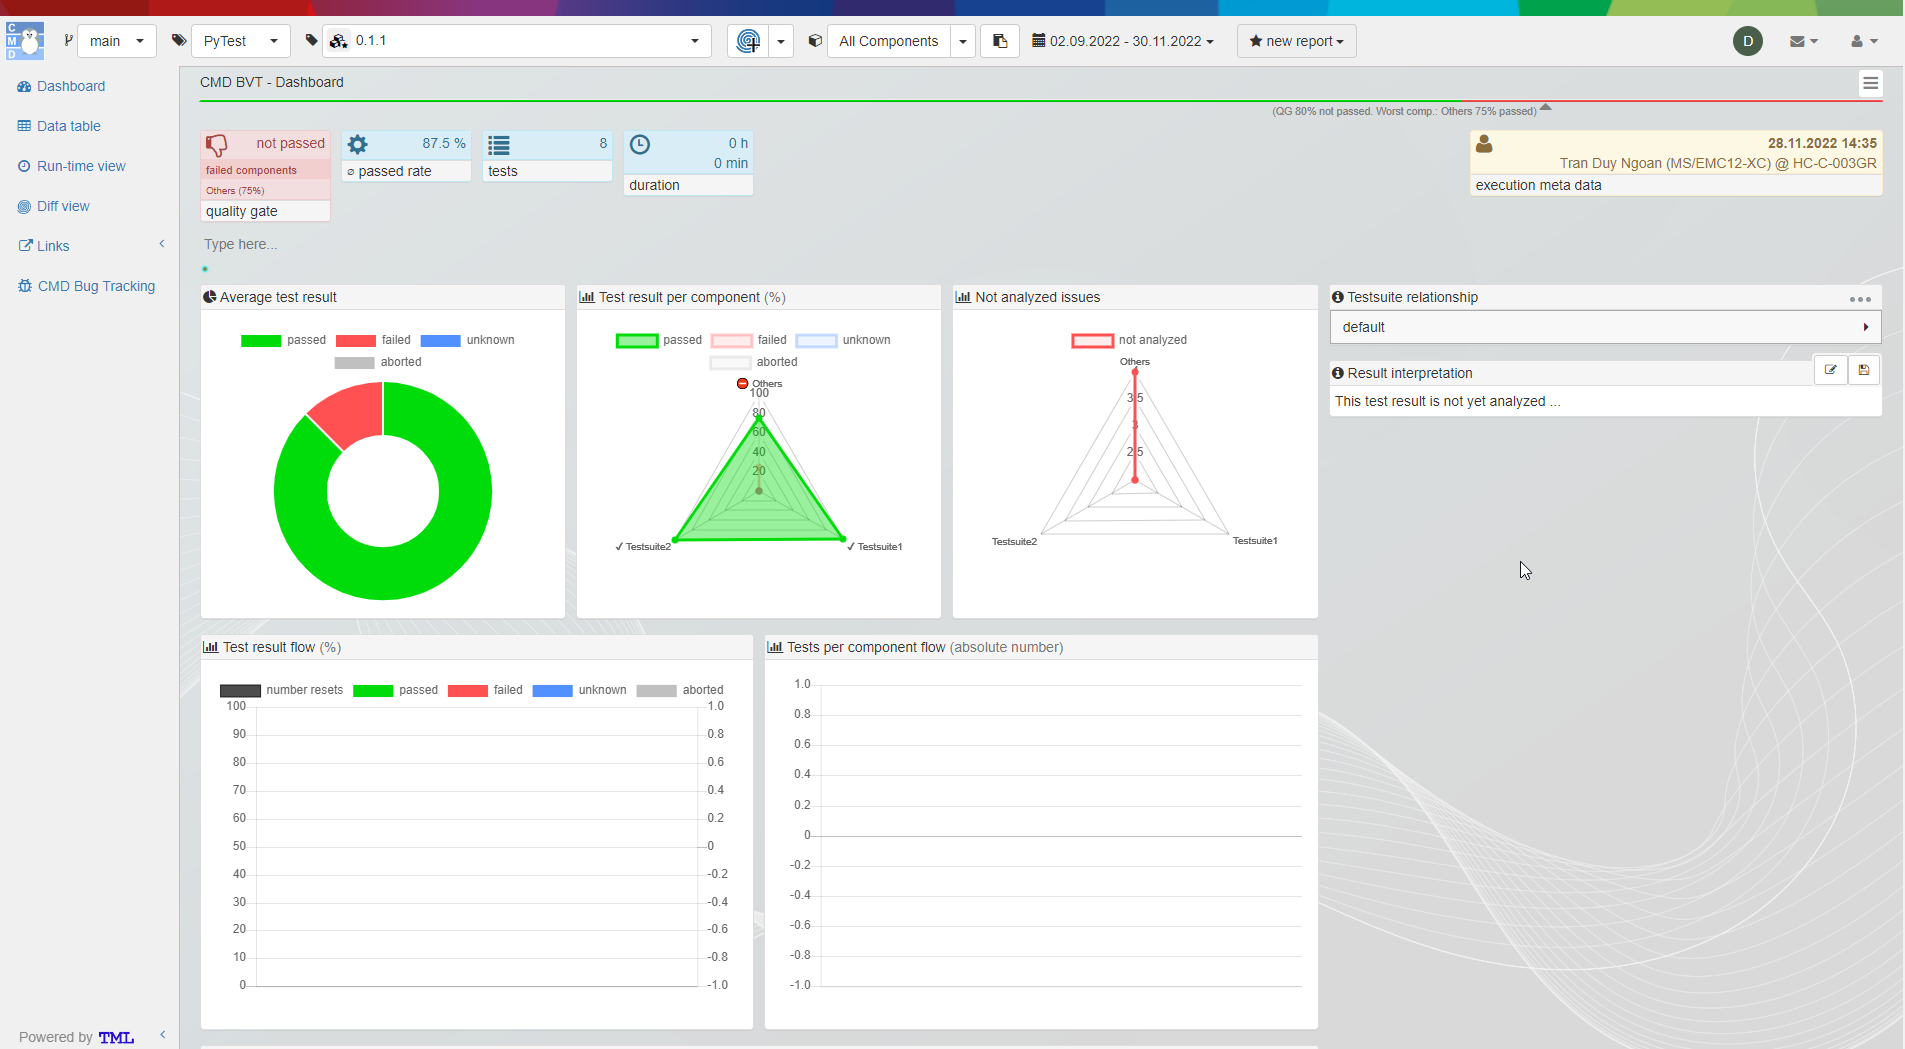
\includegraphics[width=1\linewidth]{./pictures/Dashboard.png}
  \caption{Dashboard view}
\end{figure}

Datatable view:

\begin{figure}[h!]
  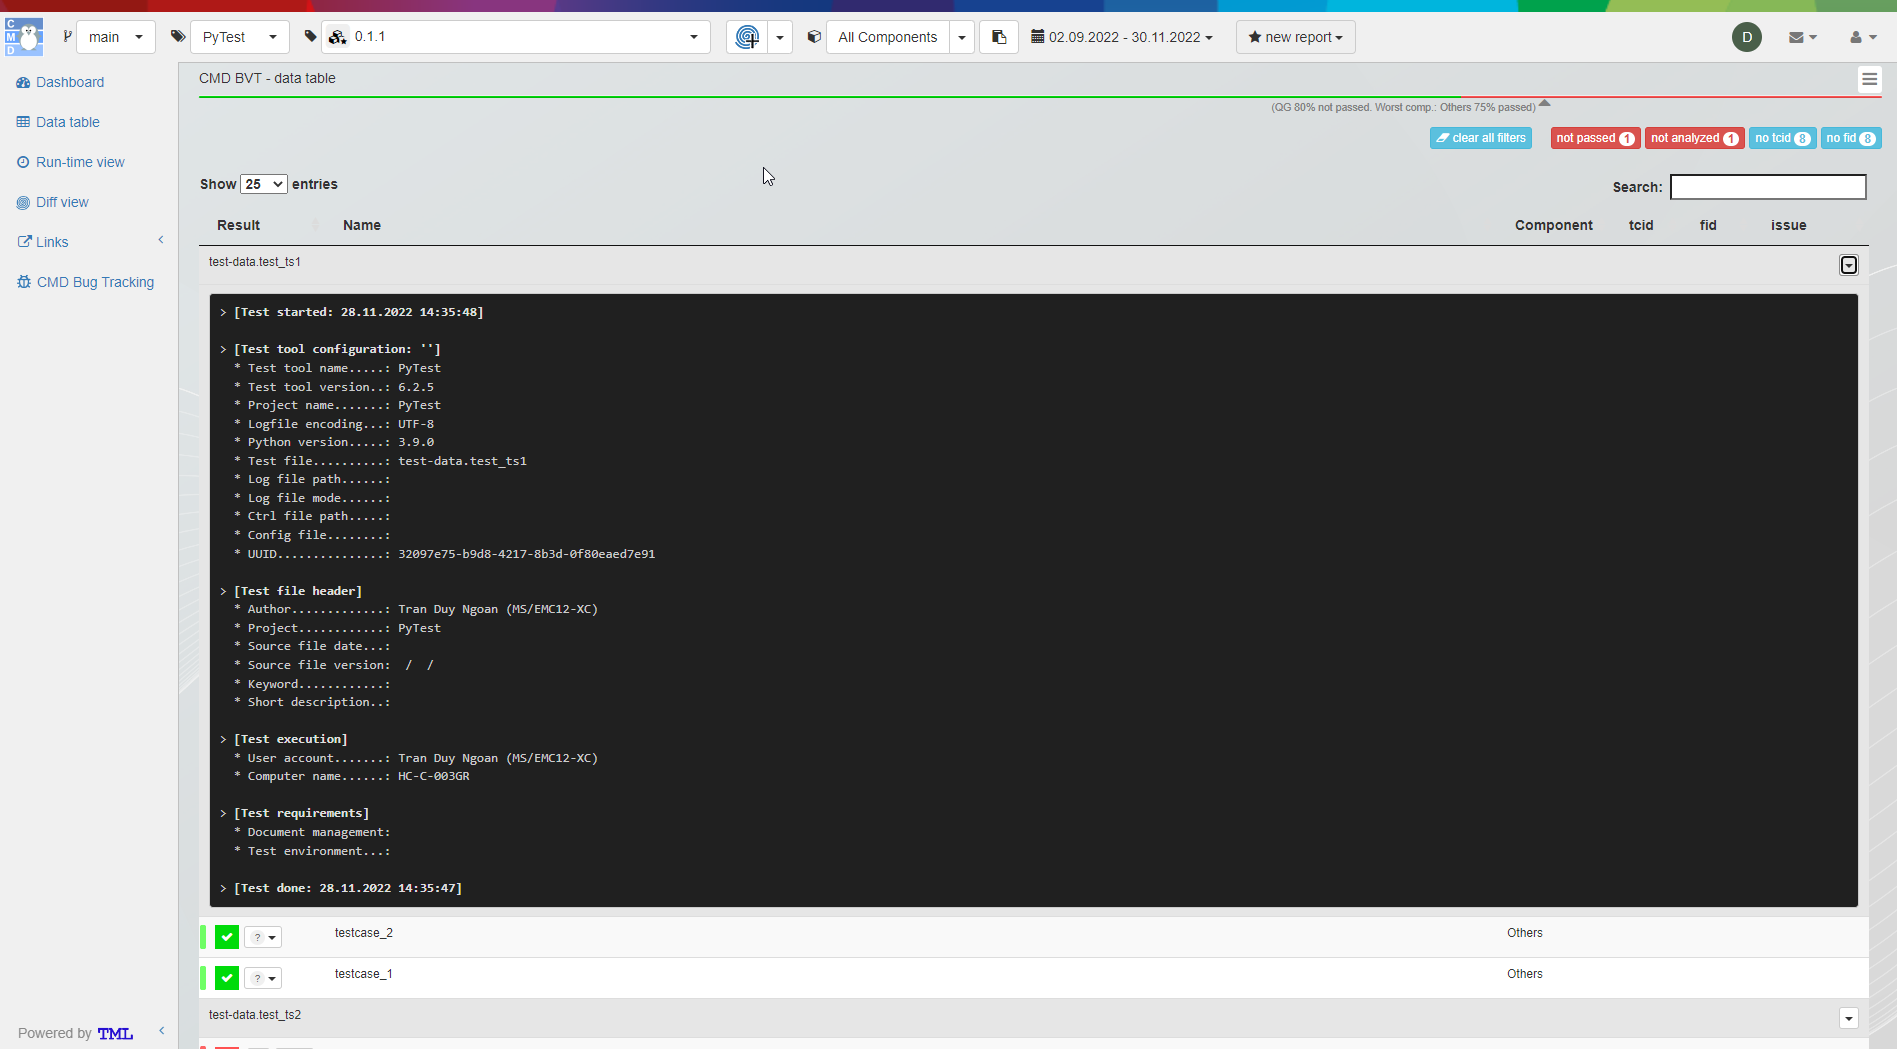
\includegraphics[width=1\linewidth]{./pictures/Datatable.png}
  \caption{Datatable view}
\end{figure}